\section{Is the Cast Operator used?}
\label{sec:casts:stats}

\newcommand{\nproject}{194}
\newcommand{\nloc}{16,329,053}
\newcommand{\nexpr}{49,886,173}
\newcommand{\nstmt}{11,410,791}
\newcommand{\ncast}{154,698}
\newcommand{\nmethod}{1,234,726}
\newcommand{\nmethodwithcast}{85,953}
\newcommand{\castpercentage}{6.74}


\newcommand{\nCastExpr}{21,491} 

To answer \ref{casts:rq1} (\emph{\crqA}),
we need the following elements:

\textbf{Source Code Analysis.}
We have gathered cast usage using the \ql{} query language.
\ql{} is ``a declarative, object-oriented logic programming language for querying complex, potentially recursive data structures encoded in a relational data model''~\citep{avgustinovQLObjectorientedQueries2016}.
\ql{} allows us to analyze programs at the source code level.
\ql{} extracts the code sources of a project into a Datalog model.
Besides providing structural data for programs, \ie{}, ASTs, \ql{} has the ability to query static types and perform data-flow analysis.
To run our \ql{} queries, we have used the service provided by Semmle.\footnote{\url{https://lgtm.com/}} 

\textbf{Projects.} 
As a code base representative of the ``real world'',
we have chosen open-source projects hosted in \github{},
the world's most popular source code management repository.
To answer \ref{casts:rq1}, we have analyzed \nproject{} \java{} projects in \lgtm{}.

Ultimately, we want to know how many cast instances are used in a given project.
To this end, we gather the following statistics using \ql{}.
We show them here to give an estimation of the size of the code base being analyzed.
The query to gather these statistics is available in Appendix~\ref{cha:ap:qlstats}.

\begin{center}
\begin{tabular}{lr}
	\hline
	Number of Projects & \nproject \\
	Number of LOC & \nloc{} \\
	Number of Methods & \nmethod \\
	Number of Methods \emph{w/}Cast & \nmethodwithcast \\
    Number of Expressions & \nexpr \\
    Number of Cast Expressions & \nCastExpr \\
	\hline
\end{tabular}
\end{center}

The \emph{Number of Methods} and \emph{Number of Methods w/Cast} values includes only methods with a body, \ie{}, not abstract, nor native.
The \emph{Number of Expressions} value shows how many expressions there are in the ASTs of all source code analyzed, \eg,
the AST of the expression $(1+2)+3$ contains 5 expressions: 2 add and 3 literal expressions.
Finally, the \emph{Number of Cast Expressions} value indicates how many cast expressions (subtype of \code{Expr} as defined by \ql{}) were found.

For our study, we are interested in both upcasts and downcasts.
We are also interested in widening primitive conversions
(Section~$5.1.2$ from the \java{} Language Specification~\citep{Gosling:2013:JLS:2462622}).
We \emph{exclude} narrowing primitive conversions in our study
(Section~$5.1.3$ from \cite{Gosling:2013:JLS:2462622}).
Primitive conversions are always safe in terms of throwing \code{ClassCastException}.
A primitive conversion happens when both the type of the expression to be cast and the type to cast to are primitive types.
Note that with this definition, we include in our study \emph{boxed} types.
Since boxed types are reference types (and therefore not necessarily safe)
we want to include them in our analysis.

We want to know how many cast instances there are across projects.
Thus, we have computed the ratio between methods containing
at least a cast over total number of methods --- with implementation --- in a given project.
The following chart shows this ratio for all analyzed projects:

\begin{figure}[ht!]
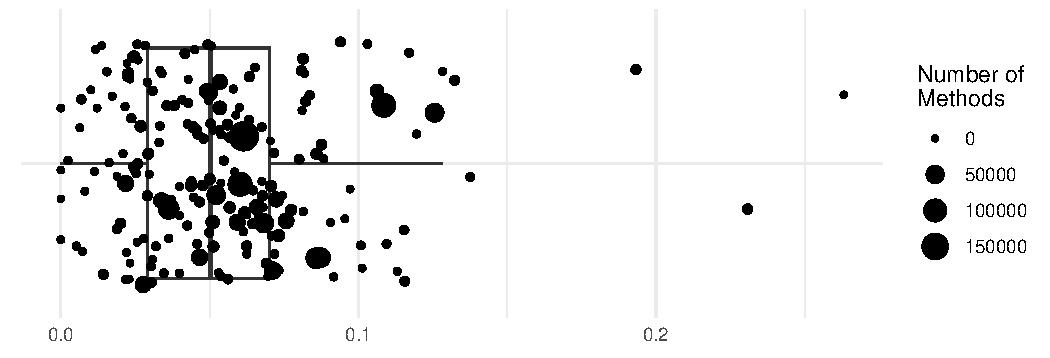
\includegraphics[width=0.9\columnwidth]{stats/stats-methodwcastXproject.pdf}
\caption{Methods with casts over total number of methods by project.}
\end{figure}

Each dot in the chart represents a project, and its size is given by the number of methods in the project.
All projects have less than 30\% of methods with at least a cast.
The chart shows that overall \castpercentage{}\% of methods contain at least one cast operation. 
This means there is a low density of casts.
This low density of casts can be attributed to the introduction of generics
--- parametric polymorphism~\citep{cardelliUnderstandingTypesData1985} ---
to \java{} 5 in 2004.
Parametric polymorphism allows the developer to use types as parameters when defining classes or methods. It permits more type errors to be checked at compile-time rather than run-time.
Since these type errors are checked at compile-time,
the cast operation in those situations is no longer needed.

Nevertheless, casts are still used.
We want to understand why there are cast instances (\ref{casts:rq2}) and how often the use cases that lead to casts are used (\ref{casts:rq3}).
The following sections give an answer to these questions.
